\documentclass{article}
\usepackage[utf8]{inputenc}
\usepackage{natbib}
\usepackage{graphicx}


\title{Background Reading List Analysis}
\author{Robert Twyman}
\date{October 2018}

\maketitle
\begin{document}


I will write my notes regarding the first 5 documents that Kris sent me on October 8th 2018 in an email titled "RE:reading material"

The documents are \cite{Alessio2006}, \cite{Bailey2014}, \cite{Zeng2001}, \cite{vanderVos2017}, \cite{Qi2006}

\section{PET Image Reconstruction - 
alessioPETRecon \cite{Alessio2006}}
\subsection{The model}
One way to represent the imaging system is with the following linear relationship
\begin{equation}\label{eq.model}
p = Hf + n 
\end{equation} 
= Hf + n s the set of observations, H is the known system model, f is the unknown image, and n is the error in the observations. The goal of reconstruction is to use the data values p (projections through the unknown object) to find the image f.
\subsection{Central Slice Theorem}
also known as central-slice theorem or Fourier-slice theorem is a foundational relationship found in analytically image reconstruction. The theorem states that that the Fourier transform of a one-dimensional projection $p(s, \phi)$ is equivalent to a section, or profile, $P(v_s,\phi)$ at the same angle through the center of the two-dimensional Fourier transform of the object, Fig.\ref{Fig.Central-Slice}. Here we see that the 1D projection (photon detection in the "camera") is transformed into Fourier space. The Fourier projection is equivalent to a section/profile, at the same angle and through the center, of the 2D Fourier transform of the object. If we know $P(v_s,\phi)$ for all angles $0\leq \phi \leq \pi$ then we can fill in the values of $F(v_x,v_y)$. The inverse of this 2D Fourier transform provides us with $f(x,y)$ in the patient (lab) frame.

\begin{figure} [h]
\centering
	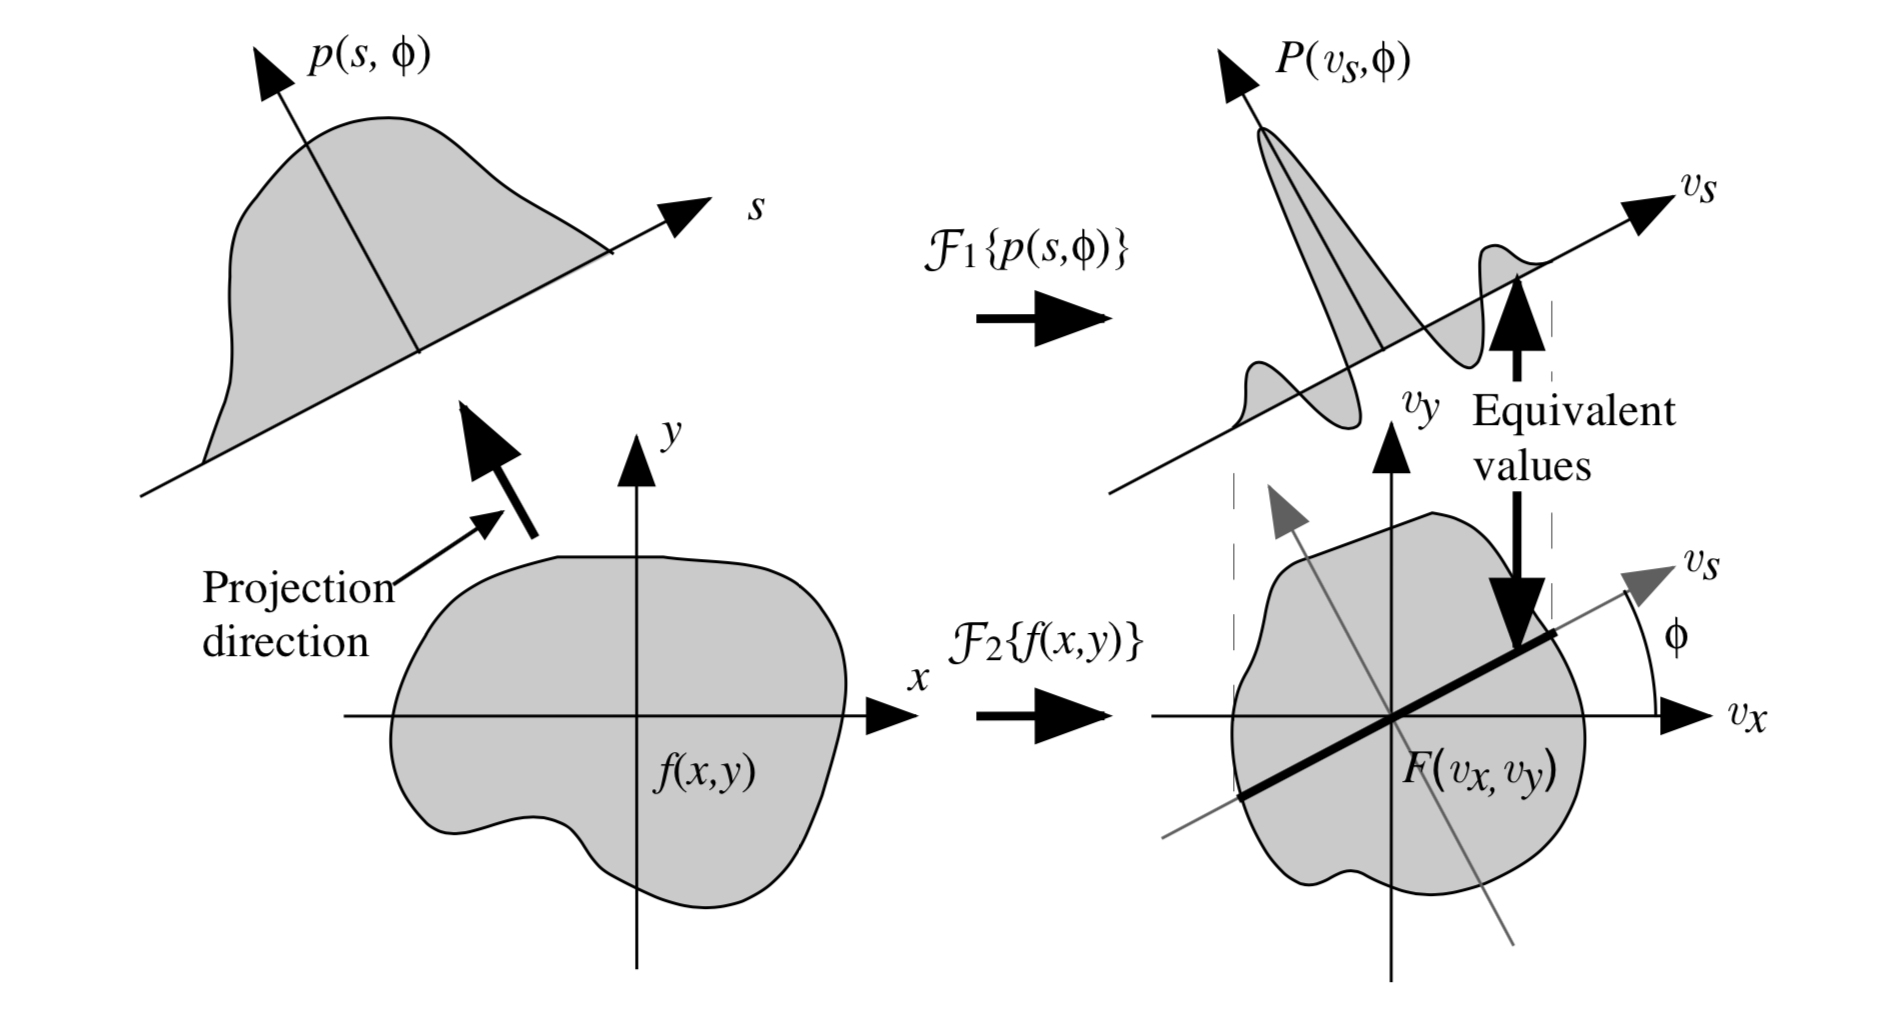
\includegraphics[width=\linewidth]{Background Reading Analysis/Central-section_theorem.png}
    \caption{\label{Fig.Central-Slice}}
\end{figure}

\subsection{Backprojection}
Backprojection is an essential step in image reconstruction. The concept of backprojection involves placing the value of $p(s,\phi)$ along the path of the respective LORs at angle $\phi$. However, because there is no knowledge as to where along the backprojection the values came from, constant values are backprojected along the LOR. This does not return the image due to oversampling in the center of the Fourier transform. 

For example: if we project back at angles $\phi_1$ and $\phi_2$ and examine the result after Fourier, we will see the contribution at the origin is double while there is only one contribution at the edges of the FOV. 
Another example: consider a single point source at the origin, the area around the origin in the reconstructed image will be heavily blurred due to the projections are added back to the entire LOR. These examples of oversampling indicate that some thing needs to be re-weighted/ filtered to obtain equal contributions. 

We can filter the Fourier transform with filter $v = \sqrt{v_x^2 + v_y^2}$ such that the Fourier transform from the backprojection $B(v_x,v_y)$ becomes:

\begin{equation} \label{eq.filtered fourier}
    F(v_x,v_y)= v B(v_x,v_y)
\end{equation}



This desensitizes the Fourier transform with a 'cone' filter. This process is know as \textbf{Backprojection Filtering (BPF)}

\subsection{Filtered Backprojection}
The filtered backprojection equation can be written as:
 \begin{equation} \label{eq.filtered backprojection}
  f(x,y) = \int_0^\pi p^F(s,\phi) d\phi
 \end{equation}
where the filtered projection is given by:
\begin{equation}
	p^F(s,\phi) = \mathcal{F}_1^{-1} \bigg\{ |v_s| \mathcal{F}_1\{ p(s,\phi)\}\bigg\}
\end{equation}
This is 'pre'-corrected for the oversampling of the Fourier transform of $f(x,y)$. 

\subsection{Regularization}
The inverse problem of Eq.\ref{eq.model} (and solving for $f$) is ill-posed and its solution Eq.\ref{eq.filtered backprojection} is unstable in the sense that a small perturbation of the data $p(s,\phi)$ can lead to unpredictable changes in the estimation of $f(x,y)$. Photon detection is stochastic and so regularization can be used to constrain the solution space to physically acceptable values.

We can add a regularization term into the \textbf{FBP} algorithm Eq.\ref{eq.filtered backprojection}:

\begin{equation} \label{eq.apodizing}
	f(x,y) \approx\tilde{f}(x,y) = \int_0^\pi \mathcal{F}_1 \big \{W(v_s) |v_s| \mathcal{F}_1 \{p(s,\phi)\}\big\}
\end{equation}
where $W(v_s)$ is a regularization/ apodizing function.
NOTE: the term "filter" in the literature is reserved for the unique "ramp" filter $|v_s|$ in tomographic image reconstruction.

\subsection{3D image reconstruction}

Two major differences between 2D and 3D image reconstruction are: 
\begin{itemize}
\item Spatially-varying scanner response - In full 3D the scanner is more sensitive to activity at the center of the axial FOV than at the edges. This is because more oblique planes intersect the center of the scanner leading to spatial variance which complicates the image reconstruction.
\item Data Redundancy - Positively - full 3D data contains redundancies due to only a single slice being required, to reconstruct an image, therefore multiple slices of the 3D data are redundant.
\end{itemize}

Spatial invariance of 3D projection data is to use a 3D re-projection algorithm. These algorithms estimate the unmeasured regions of projection by numerically forward-projecting though and estimate image. The inital estiamate is formed from reconstructing an image using only the direct planes (not truncated) with 2D FBP for each transverse plane.

\subsubsection{Rebinning}
3D x-ray transform data can be estimate a stacked (volumetric) set of 2D transverse sinograms by using signal averaging. This is known as rebinning. Each rebinning sinogram can be reconstructed with either analytic or iterative 2D reconstruction methods.
However, there is a price to pay with a penalty in spatially-varying distortion and/or amplification of noise.

Algorithms
Single-slice rebinning (SSRB) is the simplest rebinning algorithm - rebinned sinograms are formed from averaging all of the oblique sinograms that intersect the direct plane at the center of the transaxial FOV.
The Fourier rebinning (FORE) algorithm - based on  reasonably accurate equivalence between specific elements in the Fourier transformed oblique and the transverse sinograms. After normalization of for the sampling of the Fourier transform, sinograms can be recovered from the inverse transform. 
FORE amplifies statistical noise slightly over SSRB but has less distortion. 

\subsection{Iterative Image Reconstruction}

Five Basic Components

1) \textbf{Model for the image} - ie discretization of the image domain into N pixels/ 2D elements or voxels/ 3D elements

2) \textbf{Model for the system} - relate the image to the data. An element $H_{ij}$ of the system model, $\textbf{H}$ characterized the imaging system and represents the probability that an emission from voxel $j$ is detected in projection $i$. $\bar{p}_i = \sum_{j=1}^{N} H_{ij}f_j $ - where $\bar{p}_i$ is the mean of the $i^{th}$ projection and $f_j$ is the activity in voxel $j$.

3) \textbf{Model for the data} - the statistical methods describing the relationship between the value of the measurements and the expected value of the measurement. In other words - this model relates how the projection measurements vary around their expected mean values and is derived from the basic understanding of the acquisition process. Photon detection's are a Poisson distribution so this model is often used. For $M$ projections, the Poisson probability law states that the probably $\textbf{L}$ that the random vector of Poisson distributed photon counts $P$ equals the true photon counts $p$ given we have a vector of emission rates, $f$
\begin{equation}
	\textbf{L}(P=p|f) = \prod_{i=1}^M \frac{\bar{p}_i^{p_i}  e^{-\bar{p}_i}}{p_i!}
\end{equation}
If we correct for things like randoms, scatter, and attenuation, the data is no longer Poisson.
4) \textbf{Governing Principle} - Need to define the 'best' image. This is often mathematically expressed at a cost or objective function. The most common principle for iterative reconstruction is the Maximum Likelihood approach - a standard statistical estimation method which is a probability relationship. We chose an estimate of the object $\hat{f}$ that provides the greatest value of $\textbf{L}$().

Maximum-likelihood estimators are advantageous because the offer unbiased, minimum variance estimates as the number of estimates increases towards infinity. These estimators are proven to provide the least variance among all possible unbiased estimators with less noise than unbiased estimators. Due to the nature of ET and photon emission counting, the noise levels of an unbiased estimator is unacceptable so image reconstruction methods often allow some bias. This bias can be in the form of spatial smoothing - effectively adding error to the image mean values while reducing overall noise levels. This smoothing is performed either by implicitly stopping the algorithm before reaching the ML solution or explicitly through some smoothing operation (i.e. post-processing low-pass filter)

5) \textbf{An Algorithm} to optimize the cost function - Numerous algorithms have been proposed ranging from gradient decent to the more commonly used expectation maximization (EM) algorithm. A variant of this EM algorithm is the Ordered-Subsets Expectation Maximization - which is the most widely used method. 

\subsubsection{Maximum Likelihood - Expectation Maximization}
If our current ($n^{th}$) estimate of voxel $j$ is $\hat{f}^{(n)}_j$ then our future estimate will be $\hat{f}^{(n+1)}_j$

(NOTE: The next equations are generated in steps)

Forward project on all $k$ projections:
\begin{equation}
	\sum_k H_{ik} \hat{f}_k ^{(n)}
\end{equation}
Compare these estimate projections with measured projections to form a multiplicative correction factor for each projection:
\begin{equation}
	\frac{p_i}{\sum_k H_{ik} \hat{f}_k ^{(n)}}
\end{equation}
Back-project these ratios (into the image domain) to obtain a correction factor for the initial estimate:
\begin{equation}
	\sum_i H_{ij}\frac{p_i}{\sum_k H_{ik} \hat{f}_k ^{(n)}}
\end{equation}
Multiply the current image estimate by the correction estimate and divide by a weighting term based upon the system model to apply the desired strength of each image correction factor:
\begin{equation}
	\hat{f}_j^{(n+1)} = \frac{\hat{f}_j^{(n)}}{\sum_{i'} H_{i'j}}\sum_i H_{ij}\frac{p_i}{\sum_k H_{ik} \hat{f}_k ^{(n)}}
    \label{eq.ML-EMiteration}
\end{equation}
The algorithm now recenter the new estimate $\hat{f}_j^{(n+1)}$ as the new estimate and repeats.

As the EM algorithm iterative guesses an image estimate, low frequency components appear in a few iterations. As the ML estimate is approached, higher frequency  definition is resolved in the image - effectively adding more variance to the reconstructed image. As previously mentioned, the variance can be reduced with early-stopping or by post-smoothing the reconstruction. 

While the convergence rate of the image reconstruction is image dependant, it typically takes between 20 and 50 iterations to reach an acceptable solution. Considering the ML-EM algorithm requires a forward and backward  projection at each iteration, the overall processing time is much greater than that of the filtered backprojection approach aforementioned but leads to a potentially more accurate reconstruction. 

\subsubsection{Ordered Subsets Expectation Maximization (OSEM)}
Aims to reduced reconstruction time of conventional ML-EM by breaking the data into subsets.
\begin{equation}
	\hat{f}_j^{(n+1)} = \frac{\hat{f}_j^{(n)}}{\sum_{i'\in S_b} H_{i'j}}\sum_{i \in S_b} H_{ij}\frac{p_i}{\sum_k H_{ik} \hat{f}_k ^{(n)}}
    \label{eq.OSEMiteration}
\end{equation}
This image update algorithm only differs to ML-EM via the backprojection steps sum over the projections in a subset $S_b$ in a total of $B$ subsets. An image is updated after $B$ sub-iterations as each of the subsets are iterated. If $B=1$ then OSML is the same as ML-EM.

There are different approaches for organization of projection space subsets.


\subsection{Bayesian/Penalized Methods}
Bayesian methods attempt to improve image quality by taking advantage of knowledge of the image:
\begin{itemize}
\item non-negative tracer concentrations
\item only small variation between neighboring voxels
\end{itemize}
This information is known \textit{a priori} and using Bayes' Rule, is often incorporated into a maximum \textit{a posteriori} (MAP) objective function. This objective function includes all the available information after the reception of \textit{a priori} knowledge of the image.

On the basic level, the image estimates in the iterative process are a "prior" term and leads to the guarantee of convergence with certain algorithms. Therefore, these methods are equivalent to using a "penalty" term at each iteration and these methods are also termed penalized.

The prior penalty term can promote desired properties in the image such as smoothness, edges, or even particular structure based upon anatomical information from separate CT/MR studies.

One significant challenge when applying prior/penalty terms is choosing a strength parameter that varies the influence, or strength, the penalty will have on the image. 

This leads to more complex implementation and although these Bayesian methods are starting to see clinical implementation, they are slow to uptake these methods due to the challenge of choosing an appropriate parameter for governing the strength of the penalty term.


\subsection{3D Iterative Reconstruction}

Conceptually, the same iterative methods can be extended to fully 3D PET measurements and reconstruction as previously mentioned for the 2D images. The difference is the image model is now a 3D volume with voxels instead of a 2D image with pixels.

The primary challenge for 3D PET reconstruction is the major increase in computational demand. 
\begin{itemize}
\item The image sizes increase from $10^4$ pixels to $10^5$ voxels.
\item The dataset increases from $10^4$ to as much as $10^7$ entries. 
\item The system model must be computed for effectively $10^{12}$ combinations (instead of $10^8$ for 2D PET)
\end{itemize}
A further option for the iterative methods is to first re-bin the 3D data into 2D transaxial slices (as aforementioned) then proceed with the faster 2D iterative reconstruction processes.

\subsection{Definitions of Image Quality}
There is a challenge in tomographic reconstruction techniques - which method of reconstruction provides the 'best' image. Two of the major imaging task categories are classification tasks and estimation tasks. Classification tasks categorize the image or features in the image into one or more classes. A common classification task is detection (a binary classification task). Some other examples of classification tasks include signal detection, image segmentation, and diagnosis. On the other hand, estimation tasks seek numerical parameters from an imaging system such as the quantitation of physiological parameters or the estimation of features for pattern recognition. Specific examples of estimation tasks include a cardiac ejection fraction or the value of tracer flux in a tissue compartment model.

One common approach to assess image quality is to look at figures of merit  such as: signal to noise ratio, bias, contrast levels etc. However care must be taken when assessing these measures as the image volume of $10^6$ elements is described by just a few descriptor values. 

Another trade-off is in image quality is bias vs. variance. PET data is random - meaning if you imaged the same object multiple times, the reconstructed images would differ due to statistical variations in the model. We would prefer to have a reconstruction method which creates an image that is on average the true image: an unbiased method. That being said, we would prefer a reconstruction method that creates and image whose values do not deviate from their mean values: a zero variance method.
\begin{itemize}
\item Bais is a measure of the accuracy of our reconstruction on average
\item Variance is a measure of the precision of the estimate.
\item Thank to the target board example.
\end{itemize}


\newpage
\section{Nuclear Medicine Physics: A Handbook for Teachers and Students \cite{Bailey2014}}

\subsection{Chapter 13: Image Reconstruction}
This is known as an inverse problem - it is harder to make software to compute the true tracer distribution from photon data than to simulate tracer distribution and predict photon acquisition. As other books have mentioned, there are really two ways to reconstruct and image - analytically using mathematical inversion and iterative...



The FBP algorithm. This algorithm involves the following steps:

\begin{enumerate}
\item apply 1-d Fourier transform to $y(s, φ)$ to obtain $(F_1y)(ν, φ)$;
\item filter $(F_1y)(ν, φ)$ with the so-called ramp filter |ν|;
\item apply the 1-d inverse fourier transform to obtain the ramp filtered projections
\item apply the back-projection operator eq. (13.2) to Y(s,) to obtain the desired image Λ(x, y).
\end{enumerate}









\newpage
\section{Image Reconstruction - a tutorial \cite{Zeng2001ImageTutorial}}

2D pictures of a 3D object are the projections. The image reconstruction process takes these projections and tries to determine an image of the object.  

The rest of this document was well covered in Alessio's document \cite{Alessio2006} 






\newpage

\bibliography{ref.bib} 
\bibliographystyle{plain}\bibliographystyle{plain}

\end{document}